\subsection{Sample and descriptive distributions}

All 500 sampled personas produced valid baseline and outcome responses. Each randomized condition contains 125 outcomes. The median inferred financial-literacy score was 5. The distribution of the ordinal outcome is displayed in Figure~\ref{fig:distribution}.

Missing demographic fields were retained rather than imputed: age (465), gender (0), education (0). These fields were not required by the prespecified primary model.

\begin{table}[htbp]
\centering
\small
\caption{Descriptive willingness to invest by randomized condition}
\begin{tabular}{llrrrr}
\toprule
Market & Disclosure & $N$ & Mean & SD & Median\\
\midrule
Bear & Standard & 125 & 2.39 & 0.93 & 2\\
Bull & Standard & 125 & 3.98 & 0.98 & 4\\
Bear & XAI & 125 & 3.15 & 1.01 & 3\\
Bull & XAI & 125 & 4.97 & 0.82 & 5\\
\bottomrule
\end{tabular}
\par\smallskip
\begin{minipage}{.96\linewidth}\footnotesize Means summarize the coded 1--7 scores. The primary model treats the outcome as ordinal.\end{minipage}
\end{table}

\begin{figure}[htbp]\centering

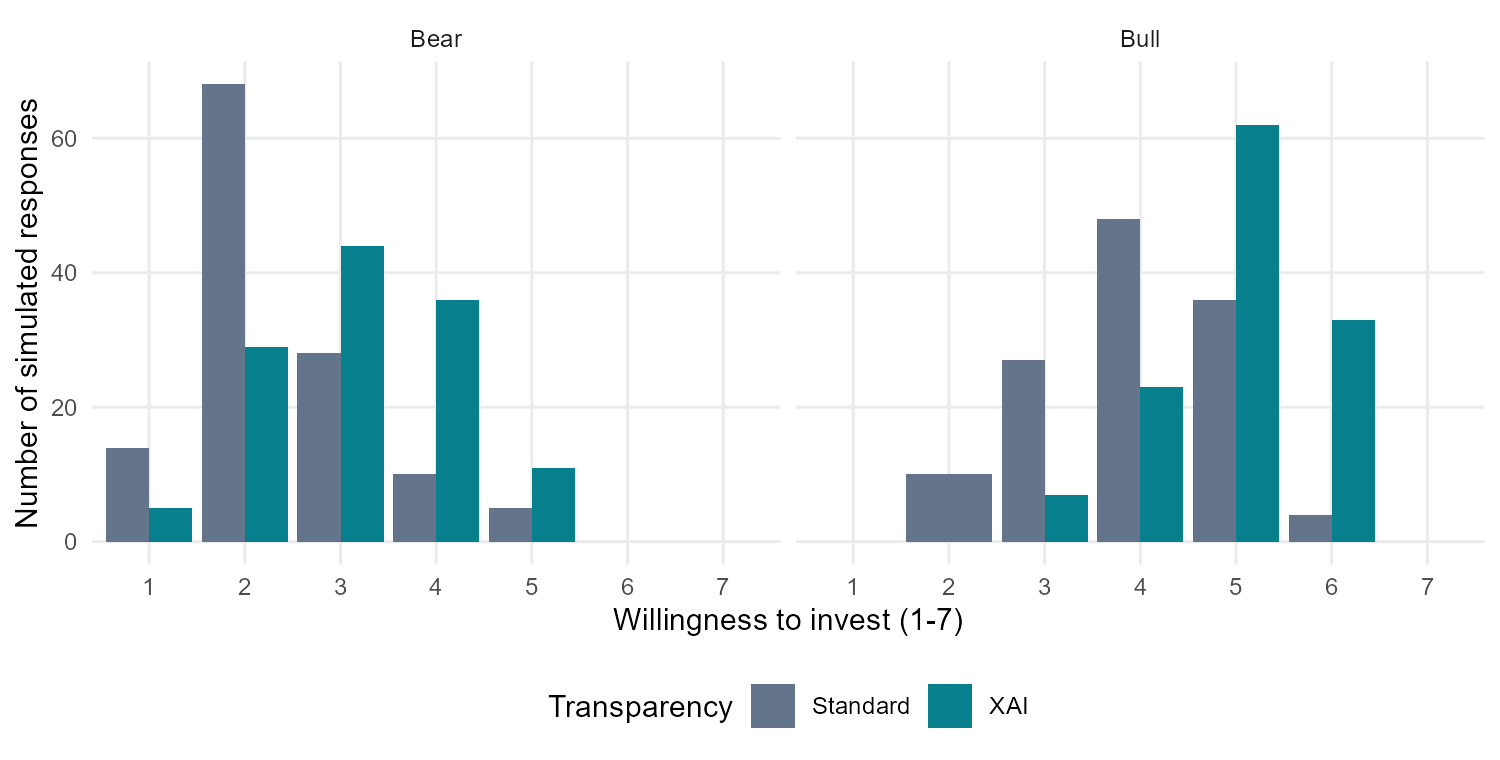
\includegraphics[width=\linewidth]{../results/outcome_distributions.png}

\caption{Distribution of single simulated investment responses by market and disclosure.}\label{fig:distribution}

\end{figure}

\subsection{Primary model and planned comparisons}

The likelihood-ratio test of the three-way interaction yielded $\chi^2(1)=0.90$, $p=0.344$. The new data therefore do not provide clear statistical support for the joint-moderation expectation. A nonsignificant test is not evidence of equivalence or of a zero interaction.

The maximum absolute gradient was 4.69e-10; the Hessian condition number was 315.6. Coefficient intervals in Table~\ref{tab:coefficients} are pointwise Wald intervals.

\begin{table}[htbp]
\centering
\small
\caption{Cumulative logit location coefficients\label{tab:coefficients}}
\begin{tabular}{lrrrrr}
\toprule
Term & $\beta$ & SE & OR & 95\% CI & $p$\\
\midrule
Bull market & 3.156 & 0.299 & 23.47 & [13.06, 42.19] & $<.001$\\
XAI disclosure & 1.528 & 0.275 & 4.61 & [2.69, 7.90] & $<.001$\\
Literacy (centered) & 0.157 & 0.107 & 1.17 & [0.95, 1.44] & 0.141\\
Market $\times$ XAI & 0.361 & 0.390 & 1.44 & [0.67, 3.08] & 0.354\\
Market $\times$ Literacy & -0.203 & 0.152 & 0.82 & [0.61, 1.10] & 0.184\\
XAI $\times$ Literacy & 0.057 & 0.154 & 1.06 & [0.78, 1.43] & 0.713\\
Market $\times$ XAI $\times$ Literacy & 0.203 & 0.214 & 1.22 & [0.81, 1.86] & 0.344\\
\bottomrule
\end{tabular}
\par\smallskip
\begin{minipage}{.96\linewidth}\footnotesize Reference conditions: bear market and standard AI. Literacy is centered at 4. With interactions, lower-order coefficients are conditional effects at the reference values. ORs for interaction terms are ratios of odds ratios.\end{minipage}
\end{table}

\begin{table}[htbp]
\centering
\small
\caption{Planned XAI versus standard-AI contrasts}
\begin{tabular}{lrrrrl}
\toprule
Market & Literacy & OR (XAI/Std.) & 95\% CI & $p_{\mathrm{Holm}}$ & Extrap.\\
\midrule
Bear & 2 & 4.11 & [1.57, 10.77] & 0.007 & No\\
Bear & 4 & 4.61 & [2.69, 7.90] & $<.001$ & No\\
Bear & 6 & 5.16 & [2.78, 9.58] & $<.001$ & No\\
Bull & 2 & 3.94 & [1.57, 9.89] & 0.007 & No\\
Bull & 4 & 6.61 & [3.82, 11.43] & $<.001$ & No\\
Bull & 6 & 11.11 & [5.74, 21.49] & $<.001$ & No\\
\bottomrule
\end{tabular}
\par\smallskip
\begin{minipage}{.96\linewidth}\footnotesize Holm correction covers all six tests. Confidence intervals are pointwise, without multiplicity adjustment. Extrapolation means that the proxy value is outside the observed range in at least one compared treatment cell.\end{minipage}
\end{table}

6 of the six planned contrasts were statistically detectable after Holm correction and within the observed cell ranges. The direction and magnitude of each comparison are shown in the table; significance differences across subgroups do not themselves establish an interaction.

The nominal-effects diagnostics flagged departures from proportional odds for 3 candidate terms at the unadjusted .05 level. Consequently, the common-odds-ratio interpretation is approximate. These diagnostic tests can be unstable in sparse categories and were not used to select a replacement primary model. Full diagnostics accompany the replication files.

2 diagnostic comparisons could not be estimated. These unavailable tests provide no evidence for or against proportional odds.

\subsection{Sensitivity analyses}

The corresponding OLS three-way coefficient was 0.075 (HC3 SE = 0.110; $p=0.498$). This is a sensitivity check on the coded score scale, not an ordinal-model estimate.

The median-split ART sensitivity test yielded $F(1,492)=0.86$, $p=0.355$. The low/high literacy group sizes are reported below; no balanced allocation was imposed on this nonrandomized moderator.

\begin{table}[htbp]
\centering
\small
\caption{Descriptive median-split subgroups}
\begin{tabular}{lllrrr}
\toprule
Market & Disclosure & Literacy group & $N$ & Mean & SD\\
\midrule
Bear & Standard & Low & 79 & 2.30 & 0.94\\
Bull & Standard & Low & 77 & 4.12 & 0.93\\
Bear & XAI & Low & 75 & 2.97 & 0.96\\
Bull & XAI & Low & 73 & 4.90 & 0.92\\
Bear & Standard & High & 46 & 2.54 & 0.91\\
Bull & Standard & High & 48 & 3.75 & 1.02\\
Bear & XAI & High & 50 & 3.42 & 1.03\\
Bull & XAI & High & 52 & 5.06 & 0.67\\
\bottomrule
\end{tabular}
\par\smallskip
\begin{minipage}{.96\linewidth}\footnotesize Low: literacy proxy at or below the sample median; High: above the median.\end{minipage}
\end{table}

\begin{figure}[htbp]\centering

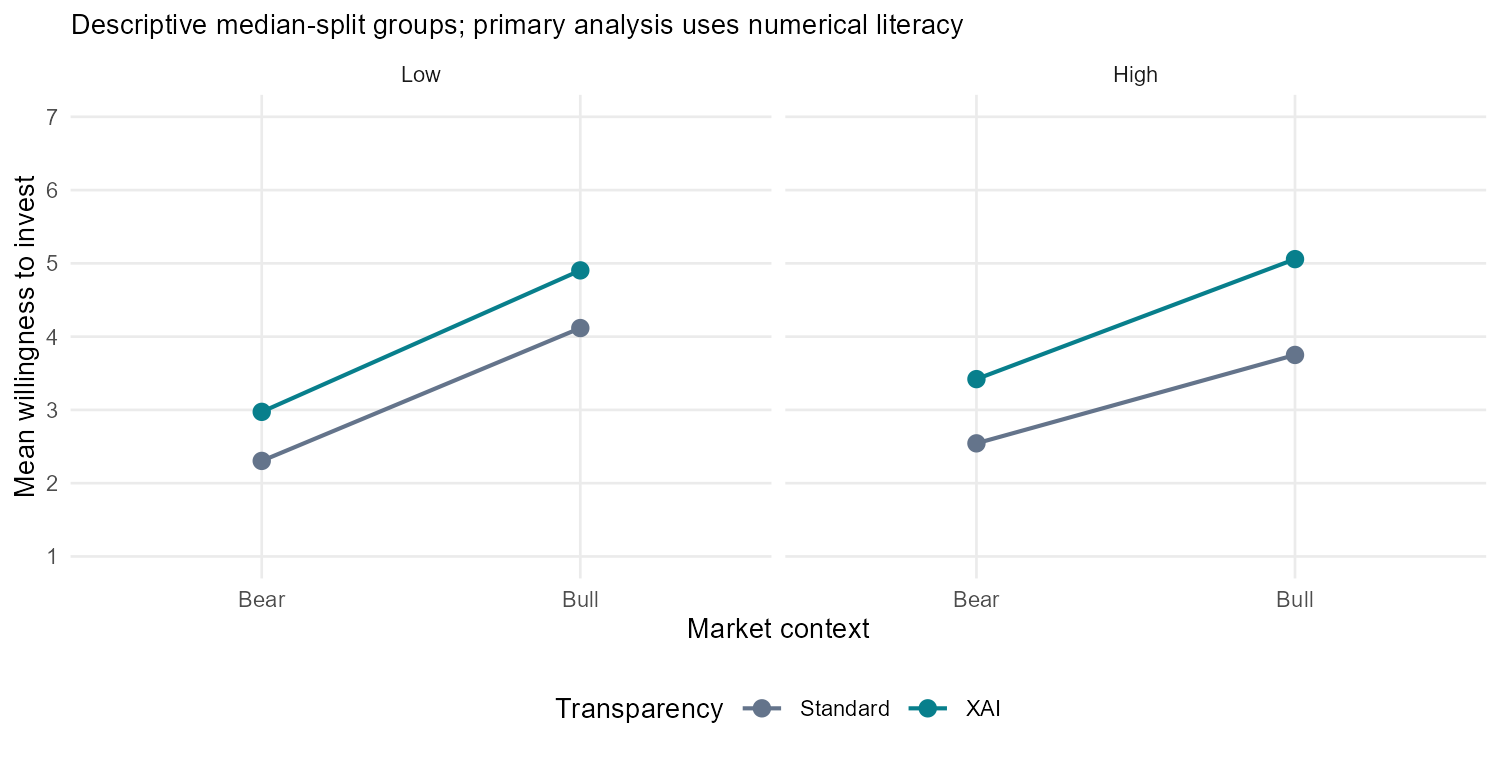
\includegraphics[width=\linewidth]{../results/interaction_descriptive.png}

\caption{Descriptive means for median-split literacy groups. The primary model retains numerical literacy.}

\end{figure}
